\section{Proposed Program}
\label{sec:pgm}

\begin{figure}[!h]
  \centering
  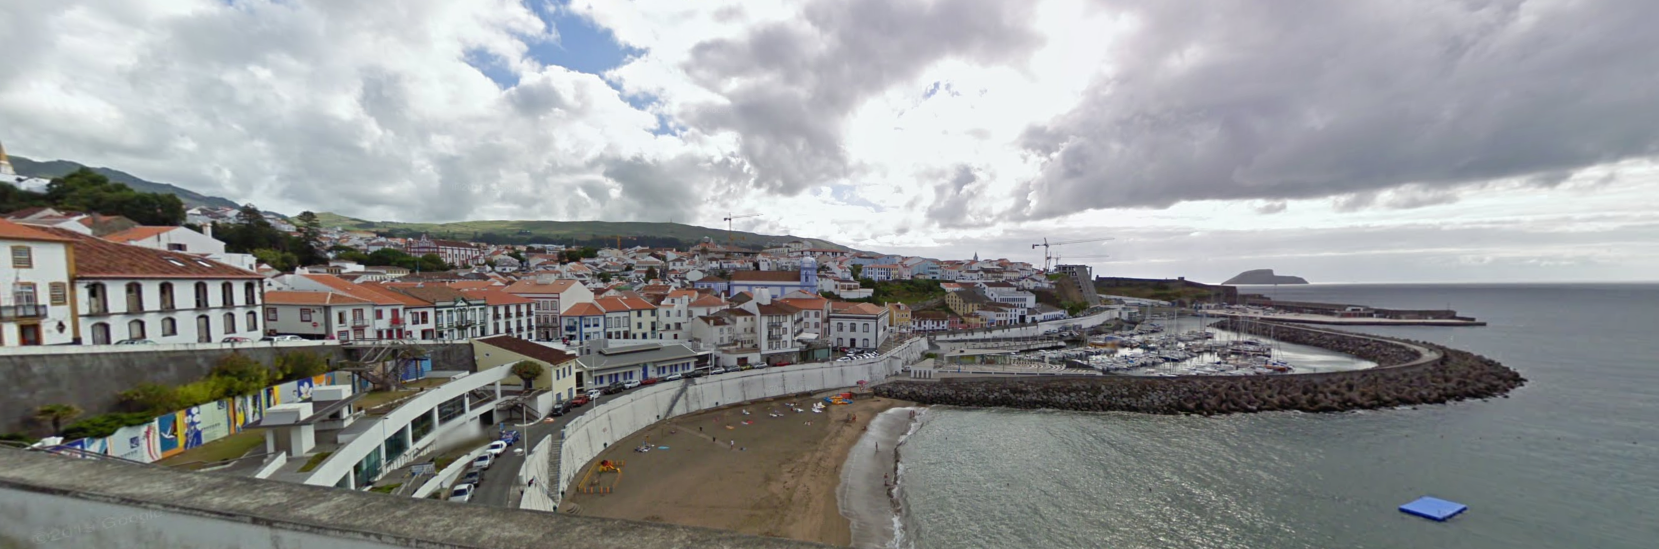
\includegraphics[scale=0.5]{fig/angra.png}
  \caption{\symp will be held in the picturesque town of Angra do
    Heroismo on Terceira Island, Azores.}
  \label{fig:angra}
\end{figure}

The \symp will be held on Terceira Island, in the Azores in the town of
Angra do Heroismo (Fig. \ref{fig:angra}). It houses the Lajes airfield,
which till recently was one of the largest military airfields outside
the US, run by the DoD and a strategic asset for long-distance
flights. Lajes is well connected to its neighboring islands, including
S\~{a}o Miguel, which enjoys direct connections to continental Europe
and to Boston and New York. Frequently run ferries also connect the
islands, although the pandemic has likely had an impact. The island
offers few distractions other than connecting with the ocean and to
nature, and therefore is an ideal setting for this event.

Angra itself is a picturesque small town and also houses the
headquarters of \aire~\footnote{\url{https://www.aircentre.org/}} which
will be the official host of the symposium. The Center will host a web
site with necessary information for the select attendees, and also
provide support during the event. A local organizer is already working
with the organizers to scout out potential hotel locations where all
attendees will be housed and will hold the meeting as well. 

\paragraph{Rules \& timing} The \symp will be based on the
\texttt{Chatham House
  Rule}\footnote{\url{https://en.wikipedia.org/wiki/Chatham_House_Rule}}
and will require everyone to respect the ideas brought forth and not
take those ideas outside the meeting. Additionally, we are anticipating
that the pandemic situation would have eased by late Spring, early
Summer (June or July) in 2022 and expect this event to be solely
in-person.

\paragraph{COVID protocol} The organizers will ask all attendees to be
vaccinated prior to the event, with an European Medicines
Agency-approved vaccine and follow European Union protocols at the time
of the event. Given the uncertain nature of the pandemic, we will target
the Spring/early Summer date, while keeping our options open to hold it
in the Fall, should there be unforeseen circumstances associated with
the pandemic. In large part, we are expecting stability in viral
caseload in holding the meeting at this time and doing so in-person
particularly because we value the person-to-person contact and
networking and the serendipitous connections we expect, that simply
cannot replace a virtual event. The organizers will closely monitor the
situation prior and during the event, to ensure this event is safe for
all and focused on the science.

\begin{table}[!t]
  \centering
  % \vspace{-0.5cm}
  \begin{tabular}{|p{2.5cm}|p{2.5cm}|p{2.5cm}|p{2.5cm}|p{2.5cm}|}
    % \multicolumn{1}{l}{r}}{l}{l}
    \hline 
    \rowcolor{Gray}
    \bfseries Day 0& \bfseries Day 1&\bfseries Day 2 &\bfseries Day 3 &\bfseries Day 4\\
    \hline
                   &Morning Session 1&Morning Session 1&Morning Session 1&Morning Session 1\\
    \hline
                   &Coffee Break&Coffee Break&Coffee Break&Coffee Break\\
    \hline    
                   &Morning Session 2&Morning Session 2&Morning Session 2&Morning Session 2\\
    \hline
                   &Lunch&Lunch&Lunch&Lunch\\
    \hline
                   &Afternoon Session 1&Networking \& Outing&Networking \& Outing&Afternoon Session 1\\
    \hline
                   &Coffee Break&Networking \& Outing&Networking \& Outing&Coffee Break\\
    \hline
                   &Afternoon Session &Networking \& Outing&Networking \& Outing&Afternoon Session 1\\
    \hline
                   &Break&Networking \& Outing&Networking \& Outing&Break\\
    \hline
    Evening reception \& registration&Dinner&Outing \& Dinner&Outing \&
                                                               Dinner&Farewell Dinner\\
    \hline        
  \end{tabular}
  \caption{Proposed high-level program for the \sympe.}
  \label{tab:symp}
\end{table}

A proposed layout and schedule for the \symp is showing in Table
\ref{tab:symp}. The fundamental premise at this meeting is to connect a
diverse group of thinkers in academia looking at ways to make
oceanographic measurements and understand processes, to think 'out of
the box'. In-person networking is therefore crucial to this event. The
symposium expects to provide various venues to connect, both in the
formal presentation/challenge/rebuttal part, as also bonding over meals
and outdoors activities. We plan to offer all meals together, and urge
people to mix and network outside their traditional academic comfort
zones. The outings in particular will help the participants to connect
with nature especially the ocean which can easily be accessed on
Terceira. Coffee and snacks will eb available throughout the formal
session, and breaks will be frequent and well-paced to allow people to
connect. Relaxed meals will also offer the ability for conversations to
lead to synergistic ideas and concepts, we believe. This event is not
meant to be a traditional 'talk-and-drop' but targeted towards
engagement. 
